\subsection{Object-Oriented Analysis of Problem Domain}
This subsection describes an analysis the the problem domain created according to the object-oriented methods, with regards to how a bus system currently works. We start out by creating an event table, followed by an explanation of the classes, then a class diagram for the problem domain, and lastly a behaviour diagram.

\subsubsection{Story}
\todo{Something needs fixing}
But first, a small story of what a typical bus driver does will be made in order to have something to loosely base the events and classes on. It is here to demonstrate exactly what we mean when we are talking about a bus driver, the driver is given this much attention. Giving the reader context to help with the understanding of the different classes and events in the event.

The bus driver shows up for work and starts his shift. He walks over to the bus that he will be driving and inspects the exterior of the bus to figure out if anything is wrong with it. He then starts up the bus and makes sure that everything inside the bus is also working. He checks that he has enough coins to pay back people that buy the tickets with cash, and he checks that the bus is clean. After this, he drives to the first bus stop on the route. While driving around he pays attention to the traffic and objects around him and makes sure that he does not crash into any of them, furthermore he follows all the traffic laws in Denmark. When he gets close to a bus stop he checks if any of his passengers have pressed the button signalling that they want to get off at the bus stop. If one or more passengers have done that or he can see that one or more persons are waiting for the bus at the bus stop he will pull over at the bus stop and open the doors. The passengers use the middle and bottom doors to get off the bus, if they used a digital card to check in at the front door, then they use the same card to check out at the other doors. The passengers coming through the front door can as mentioned earlier use a digital card to check themselves in, they can also use cash to pay for a ticket that the bus driver prints out to them. They can also show the bus driver their bus pass, or they can show the bus driver a digital ticket on their smartphone. In case a passenger has an invalid ticket, then the passenger will be asked to buy a new ticket or be kicked off the bus. In case the passenger is in a wheelchair, has a stroller with them or a lot of baggage, then they can enter the bus using the middle door, and then go up to the bus driver at the front door and use of the aforementioned methods to get allowed to use the bus. If a passenger is misbehaving then the passenger will get kicked off the bus, and the police might be called. Once all the passengers have gotten on/off the bus the bus driver closes the doors again, uses the blinkers to signal that he is driving back into the traffic, and then drives onward to the next bus stop. Once the shift of the bus driver is over there are 2 options. Either another driver takes over and starts his shift, or he pulls up to the end station and then lets all of the remaining passengers if any off the bus. After the bus is empty the bus driver checks the inside of the bus and makes sure that the bus is clean. After the bus is cleaned he will drive the bus over to its parking spot, turn the bus off, and then end his shift and leave work.

\todo{Should the text be slightly broken up?}

\subsubsection{Event Table}
Our event table can be seen on figure \ref{event-table}. The table contains the classes and events of the problem domain. The event table was made to provide an overview of how events and classes in the problem domain are connected.

\begin{table}[H]
\centering
\resizebox{\columnwidth}{!}{%
\begin{tabular}{|l|l|l|l|l|l|l|l|}
\hline
\diagbox{\shortstack{Events}}{Classes}& Passenger & Potential Passenger & Ticket & Bus Driver & Bus Stop & Bus Controller & Bus \\ \hline
Open/close door            &           &                     &        & x          &          & x              & x   \\ \hline
Push stop button           & x         &                     &        & x          &          & x              &     \\ \hline
See Potential Passengers   &           &                     &        & x          &          &                &     \\ \hline
Detecting obstacles        &           &                     &        & x          &          &                &     \\ \hline
Halt at bus stop           &           &                     &        & x          & x        &                & x   \\ \hline
Buy/print ticket           & x         &                     & x      & x          &          & x              &     \\ \hline
Start Bus                  &           &                     &        & x          &          & x              & x   \\ \hline
Turn bus off               &           &                     &        & x          &          & x              & x   \\ \hline
Person steps on            & x         & x                   &        &            &          &                & x   \\ \hline
Person steps off           & x         & x                   &        &            &          &                & x   \\ \hline
Maneuver the bus           &           &                     &        & x          &          & x              & x   \\ \hline
Safety handling            &           &                     &        & x          &          & x              & x   \\ \hline
Person arrives at bus stop &           & x                   &        &            & x        &                &     \\ \hline
Person leaves bus stop     &           & x                   &        &            & x        &                &     \\ \hline
Invalid ticket             &           &                     & x      & x          &          & x              &     \\ \hline
Start shift                &           &                     &        & x          &          &                &     \\ \hline
End shift                  &           &                     &        & x          &          &                &     \\ \hline
Check in                   & x         &                     & x      & x          &          & x              &     \\ \hline
Check out                  & x         &                     & x      & x          &          & x              &     \\ \hline
Starts Leaving Bus Stop            &           &                     &        & x          & x        &                & x   \\ \hline
\end{tabular}%
}
\label{event-table}
\caption{Event table}
\end{table}


\subsubsection{Classes}
The list below is made to help explain the event table seen in table \ref{event-table}.% this is fucked

\begin{itemize}
\item \textbf{Passenger:}
The passenger is a person that is riding the bus. They can press the stop button when they want to get off at the next bus stop. They can buy tickets from the bus driver using currency. And can both step on the bus, and off the bus. If they have a digital ticket, then they can scan the ticket to check in and scan the ticket again to check out, once they want to get off the bus.
\item \textbf{Potential passenger:}
A potential passenger is a person that is located at the bus stop. A person is a potential passenger as long as they remain at a bus stop. If a potential passenger step onto a bus they become a passenger, and passengers become potential passenger then they step off. The person object leaves the system then they leave the bus stop.
\item \textbf{Ticket:}
A ticket allows the passenger to ride the bus. It can either be a digital ticket or it can be a printed ticket. It is possible for a ticket to be invalid if it for an example has expired. It is used when the passenger checks in and when they check out.
\item \textbf{Bus driver:}
A bus driver is a person that is hired to drive a bus around a predefined route. The bus driver has a few tasks besides driving, which he primarily uses the Bus Controller to handle. These tasks are open/close doors, print and validate tickets, register if the stop button has been pressed and reset the button, or a potential passenger is standing at a bus stop. Besides these his primarily task is to drive the bus, and follow the route without hitting any obstacles and perform safety handling is necessary.
\item \textbf{Bus stop:}
Bus stops are predefined locations that determine that buss are allowed to stop at to set passengers off, or get potential passengers on. A bus stop contains a number of potential passengers, and if this number is greater then zero the next incoming bus will have to stop.
\item \textbf{Bus controller:}
The bus controller is the interface the bus driver uses to handle his different tasks, like opening/closing doors by the use of buttons. The different functionalities of the bus controller has already been descried in the Bus Driver so no further details will be written.
\item \textbf{Bus:}
This is the representation of the actual bus, and contain the information of the bus, hereby the physical components like wheels. The bus are controlled by the bus controller, to perform actions like turning.
\end{itemize}


\subsubsection{Class Diagram for the problem domain}
A class diagram for the problem domain can be seen in figure \ref{problem-domain-class-diagram}. This class diagram shows how the current system functions. The purpose of the class diagram were to find the different areas in the system and understand what they contained. Before deciding which parts that should be modelled in this project.

From the class diagram three areas was found to be important for the current system. These where the person, bus control, bus structure and the ticket part which is an other system. From the problem statement it was decided that bus controls and bus structure should be the main focus, and since the limitations of the project it was decided that modelling the ticket and passenger parts where out of scope, and will therefor not be a focus in this project. 

\todo{Fejl i figur, der mangler "has" fra passenger til ticket, samt arrow fra potential passenger skal væk, eftersom ikke alle har tickets}
\unsure{Del diagram op i de 4 forskellige dele, farver?}

\begin{figure}[H]
\centering
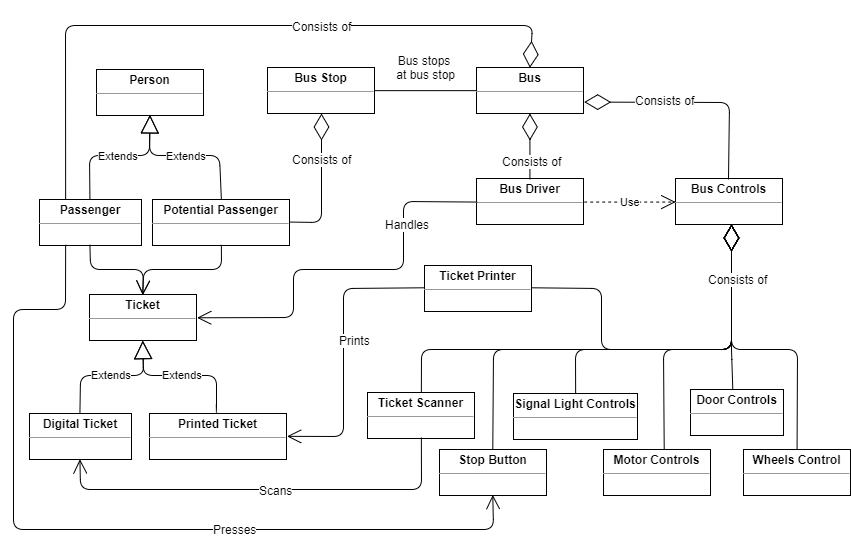
\includegraphics[scale=0.49]{Images/problem_domain_class_diagram.png}
\caption{Class diagram for the problem domain.}
\label{problem-domain-class-diagram}
\end{figure}

%Our project will mirror most of what is shown in figure \ref{problem-domain-class-diagram}, however since this project will discard the bus driver, the divers responsibilities 

\subsubsection{Behaviour Diagram}
Since a central part of the project aims to produce an autonomous bus, the bus driver's responsibilities and thereby their behaviour is relevant to our project. Figure \ref{BehaviorDiagramBusDriver} shows a state chart diagram illustrating the behaviour of the driver, events concerned the ticket and passenger part has been included for good measure. The diagram aims to illustrate the responsibilities of the bus driver and thereby show what functionality our project has to implement.

\begin{figure}[H]
\centering
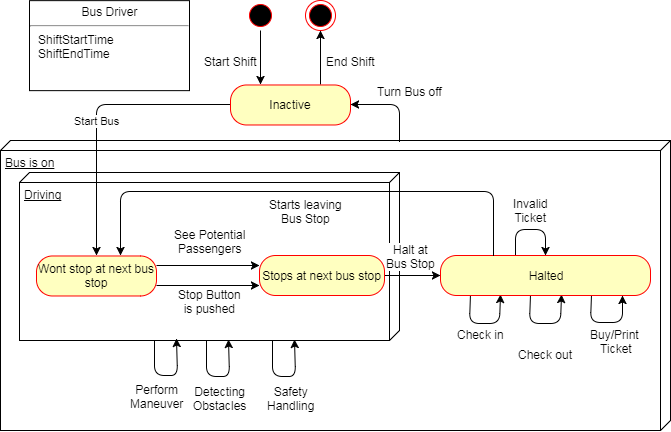
\includegraphics[scale=0.6]{Images/BehaviorDiagramBusDriver.png}
\caption{Behaviour diagram for the bus driver.}
\label{BehaviorDiagramBusDriver}
\end{figure}

% Slet?
%In figure \ref{BehaviorDiagramBusDriver} the events handling the ticket part has been included for good measure, however since we have given bus controls a higher priority, these events can mostly be ignored. This reveals some obvious knowledge the fact that the driver is the one manoeuvring, using safety handling and detecting obstacles. This is common knowledge but maybe not as easy to implement. One of the important parts of the diagram, is the fact that the driver can be in one of two states when manoeuvring. One where the driver knows it needs to stop at the next bus stop, and one where it knows it should ignore the next bus stop. 
